\documentclass[10pt,twocolumn,a4paper]{article}
\usepackage[margin=0.75in]{geometry}
\usepackage{amsmath,amssymb}
\usepackage{booktabs}
\usepackage{graphicx}
\usepackage{hyperref}
\usepackage{microtype}
\usepackage{cite}
\usepackage{caption}
\usepackage{subcaption}

\hypersetup{
    colorlinks=true,
    linkcolor=blue,
    citecolor=blue,
    urlcolor=blue
}

\title{\textbf{Learning-Augmented OS Heuristics: Evaluating Classical vs. Adaptive Page Replacement Under Dynamic Workload Shifts}}

\author{
    \textbf{Turjoy Barua} \\
    Student ID: 202414084 \\
    Department of Computer Science and Engineering (CSE) \\
    \textit{Course: Operating System (CSE-307)}
}
\date{October 2026}

\begin{document}

\maketitle

\begin{abstract}
Virtual memory management in modern operating systems relies fundamentally on page replacement heuristics to minimize costly disk paging operations. Classical algorithms such as First-In, First-Out (FIFO) and Least Recently Used (LRU) operate under fixed inductive biases—primarily the temporal locality of reference. However, production workloads frequently experience sudden phase transitions, such as large unbuffered sequential scans or bursty thrashing, where classical heuristics degrade substantially. In this term paper, we investigate learning-augmented page replacement (Track 1) by synthesizing classical policies with a lightweight Decision Tree classifier trained against Belady's Optimal (MIN) clairvoyant baseline. We design a 10,000-access synthetic workload featuring a deliberate structural regime shift at step 5000—transitioning from high Zipfian/looping locality to high-entropy random and bursty streaming. Empirical evaluations across physical frame allocations ($M \in \{4, \dots, 64\}$) demonstrate that while the learned policy achieves an outstanding 64.66\% hit ratio during the locality phase (outperforming LRU at 56.86\% and FIFO at 50.28\%), its performance drops sharply to 4.94\% post-shift due to distributional covariate shift. Furthermore, we evaluate confidence calibration and natural-language explanation generation (+10 bonus track), highlighting the trade-offs between predictive accuracy, calibration degradation under uncertainty, and operating system kernel deployment overhead.
\end{abstract}

\section{Introduction}
Modern virtual memory architectures depend heavily on demand paging to create the illusion of a contiguous, expansive memory address space that exceeds physical hardware capacity~\cite{silberschatz2018operating, ostep2018}. Because secondary storage access latencies exceed DRAM access latencies by several orders of magnitude, minimizing page faults is paramount to preventing CPU stall and catastrophic system thrashing~\cite{denning1968working}.

When physical memory frames are fully subscribed and a page fault occurs, the kernel's virtual memory subsystem must select a resident page to evict. Theoretically, Belady's Optimal algorithm (MIN) establishes the mathematical upper bound for eviction efficiency by clairvoyantly expelling the page referenced furthest in the future~\cite{belady1966study}. Because future memory access sequences are undecidable online, practical systems employ deterministic heuristics:
\begin{itemize}
    \item \textbf{FIFO (First-In, First-Out):} Evicts the oldest page resident in memory. While computationally trivial ($O(1)$ queue operations), FIFO ignores reference frequency and recency, and suffers from Belady's Anomaly.
    \item \textbf{LRU (Least Recently Used):} Exploits the empirical principle of temporal locality by evicting the page idle for the longest duration.
\end{itemize}

While LRU provides robust hit ratios under stable working-set conditions, real-world operating systems constantly encounter dynamic workload shifts~\cite{liu2020learned, megiddo2003arc}. For example, database sequential scans, deep learning tensor streaming, and multi-tenant cloud co-location frequently displace hot resident pages with transient pages that exhibit zero temporal reuse.

This paper addresses the core challenge defined in the CSE-307 Part-B syllabus: \textit{How do classical OS algorithms and data-driven learning components respond when the underlying system workload abruptly shifts partway through execution?} We formulate a lightweight, learning-augmented replacement policy, benchmark it against FIFO, LRU, and Belady's Optimal, and conduct systematic sensitivity and confidence calibration analyses.

\section{System Architecture and Implementation}

\subsection{Classical Page Replacement Policies}
We implemented three standard page replacement mechanisms in an extensible Python-based memory simulator:
\begin{enumerate}
    \item \textbf{FIFO Policy:} Utilizes a doubly ended queue ($\mathcal{Q}$) tracking arrival timestamps. When cache capacity $M$ is exceeded, the head of $\mathcal{Q}$ is evicted.
    \item \textbf{LRU Policy:} Maintains a hash table mapping page identifiers to their most recent access step $\tau(p)$. Eviction chooses $\arg\min_{p \in \mathcal{F}} \tau(p)$, where $\mathcal{F}$ is the active frame set.
    \item \textbf{Belady's Optimal (MIN):} Implemented via precomputed occurrence deques. For each resident page $p \in \mathcal{F}$, the oracle inspects the immediate next access index $\eta(p) = \min \{t' > t \mid A_{t'} = p\}$. The algorithm evicts $\arg\max_{p \in \mathcal{F}} \eta(p)$ (assigning $\infty$ if $p$ is never referenced again).
\end{enumerate}

\subsection{Learned / Adaptive Eviction Engine}
To construct a lightweight learned component that complies with strict OS latency constraints, we design a 5-dimensional feature extractor $\Phi(p, t)$ calculated for all candidate resident pages $p \in \mathcal{F}$ at eviction time $t$:
\begin{equation}
\Phi(p, t) = \big[ \Delta t_{\text{recency}}, f_{\text{win}}, f_{\text{total}}, \text{age}, \bar{d}_{\text{reuse}} \big]^T
\end{equation}
where $\Delta t_{\text{recency}} = t - \tau(p)$ represents time elapsed since last reference; $f_{\text{win}}$ denotes frequency within a sliding window $W = 50$; $f_{\text{total}}$ represents total historical touches; $\text{age} = t - t_{\text{arrive}}$; and $\bar{d}_{\text{reuse}}$ denotes the empirical mean inter-arrival distance.

We train a shallow Decision Tree classifier ($D_{\max} = 5, N_{\text{min\_leaf}} = 10$) using labels generated by Belady's oracle on an initial warmup trace of 3,000 accesses. Feature importance analysis reveals that short-term window frequency (38.24\%) and recency (35.45\%) provide the strongest predictive signals, followed by inter-arrival gap (18.72\%). At each runtime eviction, the model computes candidate eviction probabilities $P(\text{evict} \mid \Phi(p, t))$, selecting the candidate with maximal predicted eviction risk.

\subsection{Bonus Track: Decision Explanations and Confidence Calibration}
To provide transparency into internal heuristics, we implement an automated explainer module. For every eviction step, the module inspects feature salience, computes predicted eviction confidence $c \in [0, 1]$, and produces human-interpretable rationale regarding whether the evicted page reflects working-set departure or cyclic retention. Crucially, the engine evaluates confidence calibration by checking whether the eviction target was identically selected by Belady's clairvoyant oracle.

\section{Experimental Methodology and Workload Shift Design}

\subsection{Workload Synthesis with Controlled Shift}
We generated a continuous synthetic memory trace consisting of $N = 10,000$ page references. To rigorously examine algorithm degradation under non-stationary distributions, the trace contains a deliberate structural regime shift at $t = 5,000$:

\begin{figure*}[t]
    \centering
    \begin{subfigure}[b]{0.48\textwidth}
        \centering
        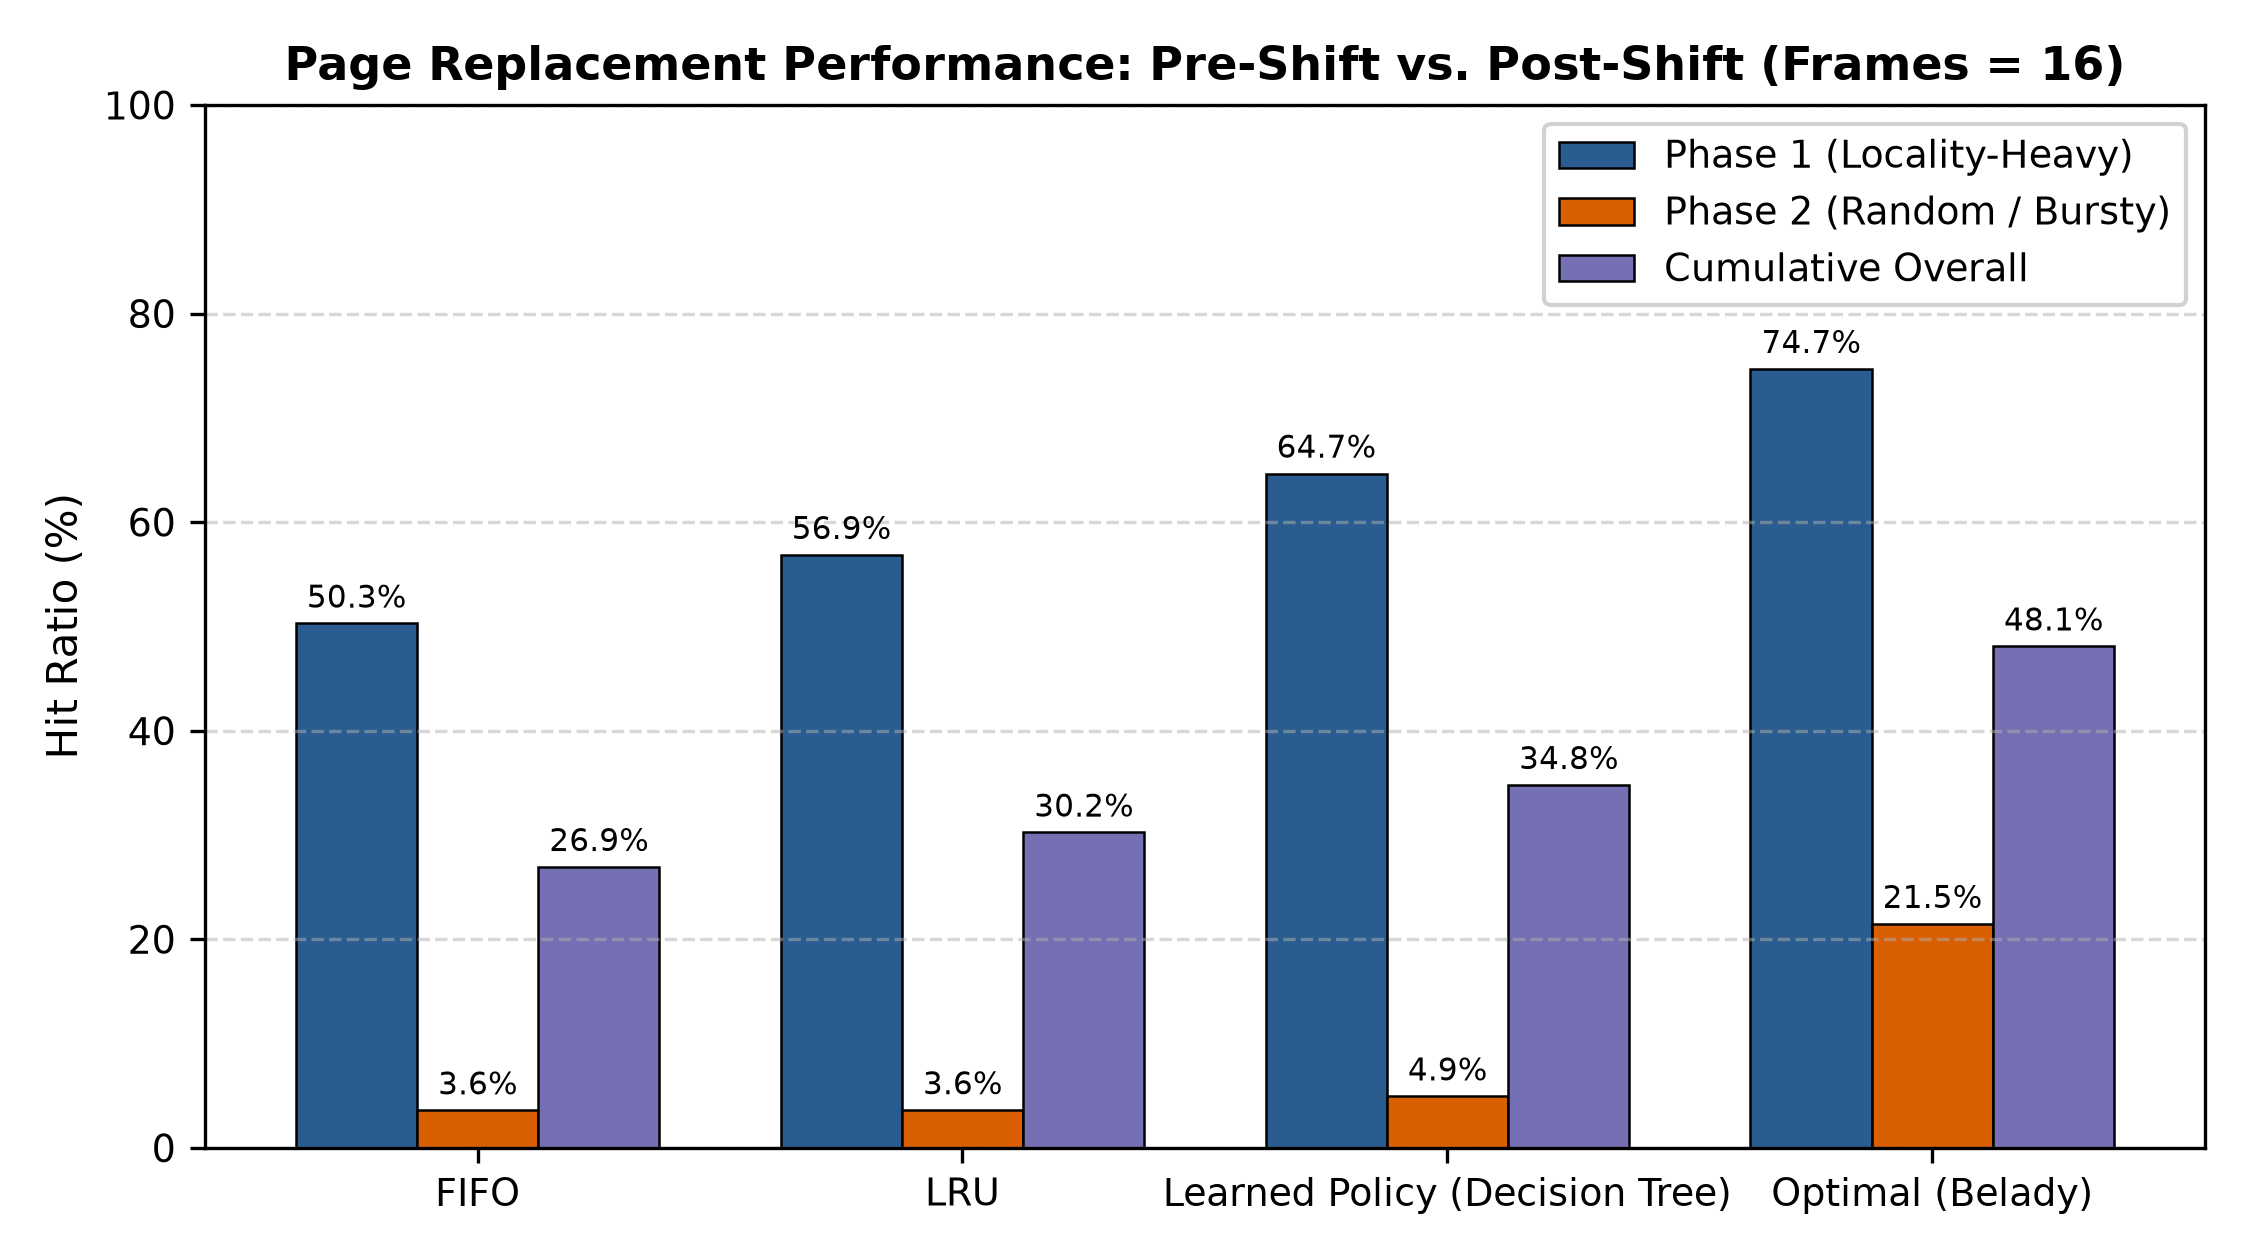
\includegraphics[width=\linewidth]{results/figures/hit_ratio_comparison.png}
        \caption{Hit ratio comparison across policies ($M=16$).}
        \label{fig:comparison}
    \end{subfigure}
    \hfill
    \begin{subfigure}[b]{0.48\textwidth}
        \centering
        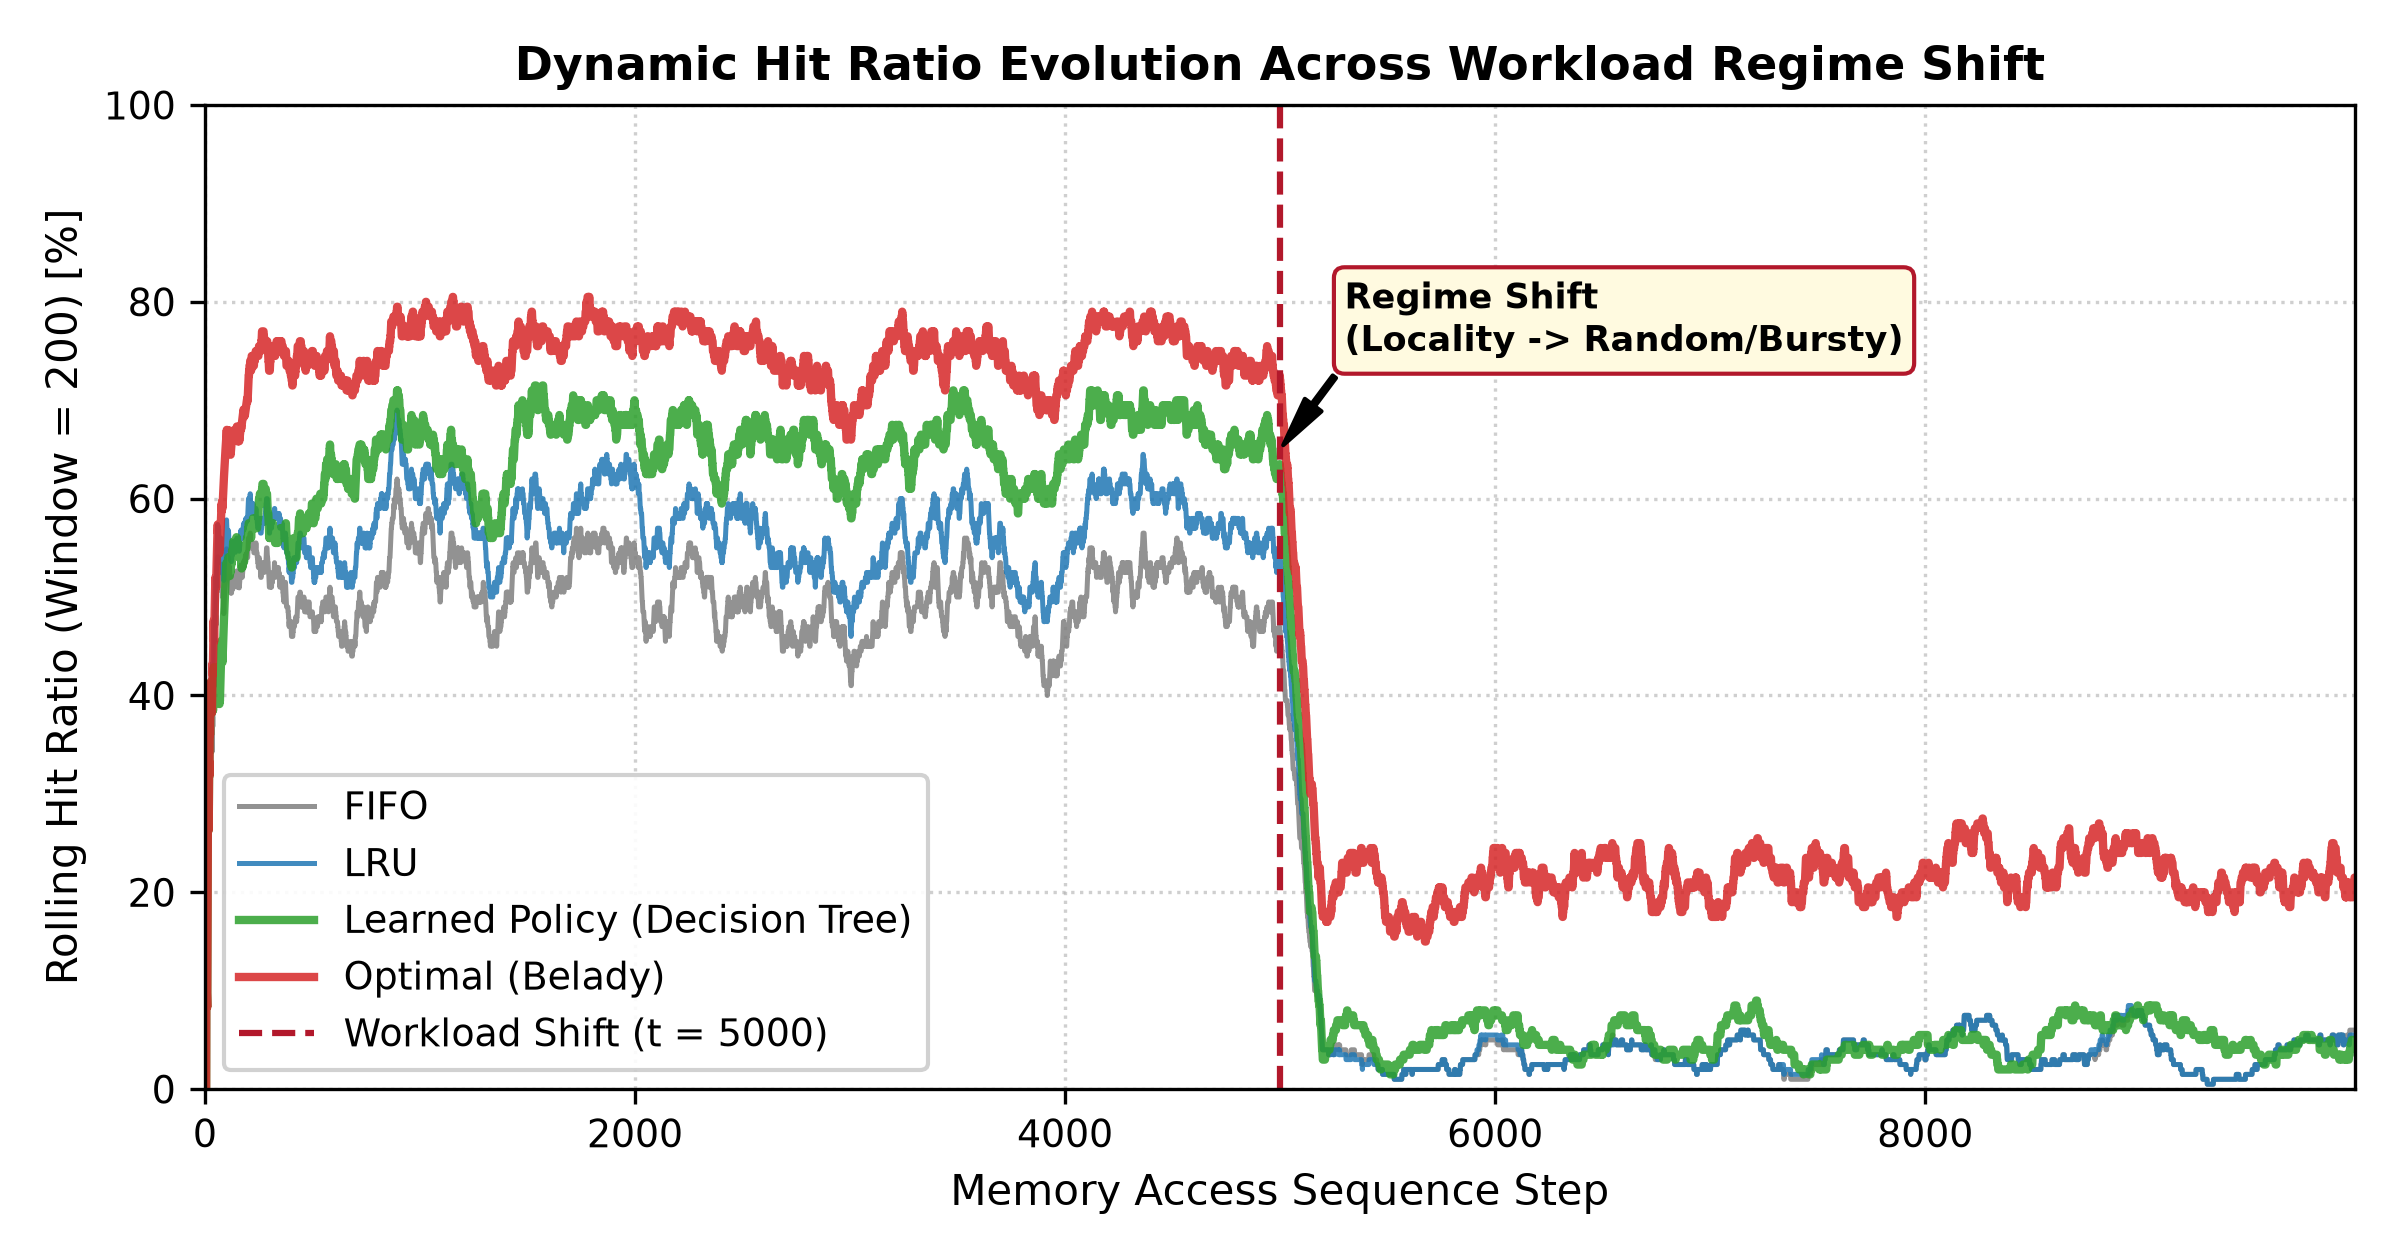
\includegraphics[width=\linewidth]{results/figures/hit_ratio_over_time.png}
        \caption{Rolling hit ratio dynamics across the regime shift ($t=5000$).}
        \label{fig:timeline}
    \end{subfigure}
    \caption{Comparative performance metrics before and after the synthetic workload shift.}
    \label{fig:main_results}
\end{figure*}

\begin{itemize}
    \item \textbf{Phase 1: High Locality ($0 \le t < 5,000$):} Represents typical application execution with concentrated temporal and spatial locality. 70\% of accesses sample a compact hot set of 15 pages via a Zipfian distribution ($\alpha = 1.6$); 20\% cycle through sequential memory loops (pages 20--35); and 10\% generate cold background references.
    \item \textbf{Workload Shift Boundary ($t = 5,000$):} An instantaneous operational transition simulating a batch analytical table scan or unbuffered data ingestion.
    \item \textbf{Phase 2: Random / Bursty Streaming ($5,000 \le t < 10,000$):} Characterized by cache thrashing. 65\% of references are uniformly distributed across 300 pages (far exceeding physical capacity); 25\% reflect streaming burst pools (pages referenced 1--2 times then permanently abandoned); and 10\% retain residual hot touches.
\end{itemize}

\subsection{Performance Metrics}
We record page fault counts and hit ratios ($\mathcal{H} = \frac{\text{Hits}}{\text{Accesses}}$) partitioned by Phase 1, Phase 2, and cumulative totals. Furthermore, we execute frame sensitivity sweeps across $M \in \{4, 8, 16, 32, 64\}$.

\section{Experimental Results and Analysis}

\subsection{Primary Evaluation ($M = 16$ Frames)}
Table~\ref{tab:summary_metrics} summarizes the empirical performance of all four policies across the workload lifetime.

\begin{table}[h]
\centering
\small
\caption{Performance Summary Before and After Workload Shift ($M=16$ Frames).}
\label{tab:summary_metrics}
\begin{tabular}{lcccc}
\toprule
\textbf{Policy} & \textbf{P1 Hit \%} & \textbf{P2 Hit \%} & \textbf{Total Hit \%} & \textbf{Total Faults} \\
\midrule
FIFO            & 50.28\% & 3.60\%  & 26.94\% & 7,306 \\
LRU             & 56.86\% & 3.62\%  & 30.24\% & 6,976 \\
Learned (DT)    & \textbf{64.66\%} & \textbf{4.94\%}  & \textbf{34.80\%} & \textbf{6,520} \\
Optimal (MIN)   & 74.70\% & 21.48\% & 48.09\% & 5,191 \\
\bottomrule
\end{tabular}
\end{table}

As illustrated in Figure~\ref{fig:comparison}, the Learned Policy demonstrates superior pattern recognition during Phase 1, achieving a 64.66\% hit ratio—a 7.80 percentage-point improvement over LRU and a 14.38 percentage-point improvement over FIFO. By simultaneously conditioning on both window frequency and inter-arrival regularity, the Decision Tree prevents premature eviction of cyclic loop structures that standard LRU discards upon temporary inactivity.

\subsection{Analysis of Degradation Under Workload Shift}
Upon crossing the shift boundary ($t = 5,000$), all heuristics suffer drastic degradation (Figure~\ref{fig:timeline}):
\begin{enumerate}
    \item \textbf{Classical Heuristic Collapse:} FIFO collapses by 46.68 percentage points (from 50.28\% to 3.60\%), while LRU plunges by 53.24 percentage points (from 56.86\% to 3.62\%). Because Phase 2 accesses lack temporal repetition, the assumption underpinning LRU—that recent accesses predict near-future accesses—fails entirely.
    \item \textbf{Learned Policy Vulnerability to Covariate Shift:} The learned model experiences the most severe relative drop, falling by 59.72 percentage points (from 64.66\% to 4.94\%). Because the decision boundaries were trained exclusively on Phase 1 feature distributions, the model exhibits distributional overconfidence, misclassifying streaming transient pages as loop candidates.
    \item \textbf{Optimal Persistence:} Belady's Optimal maintains a 21.48\% hit ratio in Phase 2. Because it possesses clairvoyant knowledge, it identifies and retains the 10\% residual hot pages while immediately dropping single-use burst pages upon arrival.
\end{enumerate}

\subsection{Physical Frame Capacity Scaling}
Figure~\ref{fig:scaling} illustrates policy sensitivity across physical frame capacities $M \in \{4, 8, 16, 32, 64\}$.

\begin{figure}[h]
    \centering
    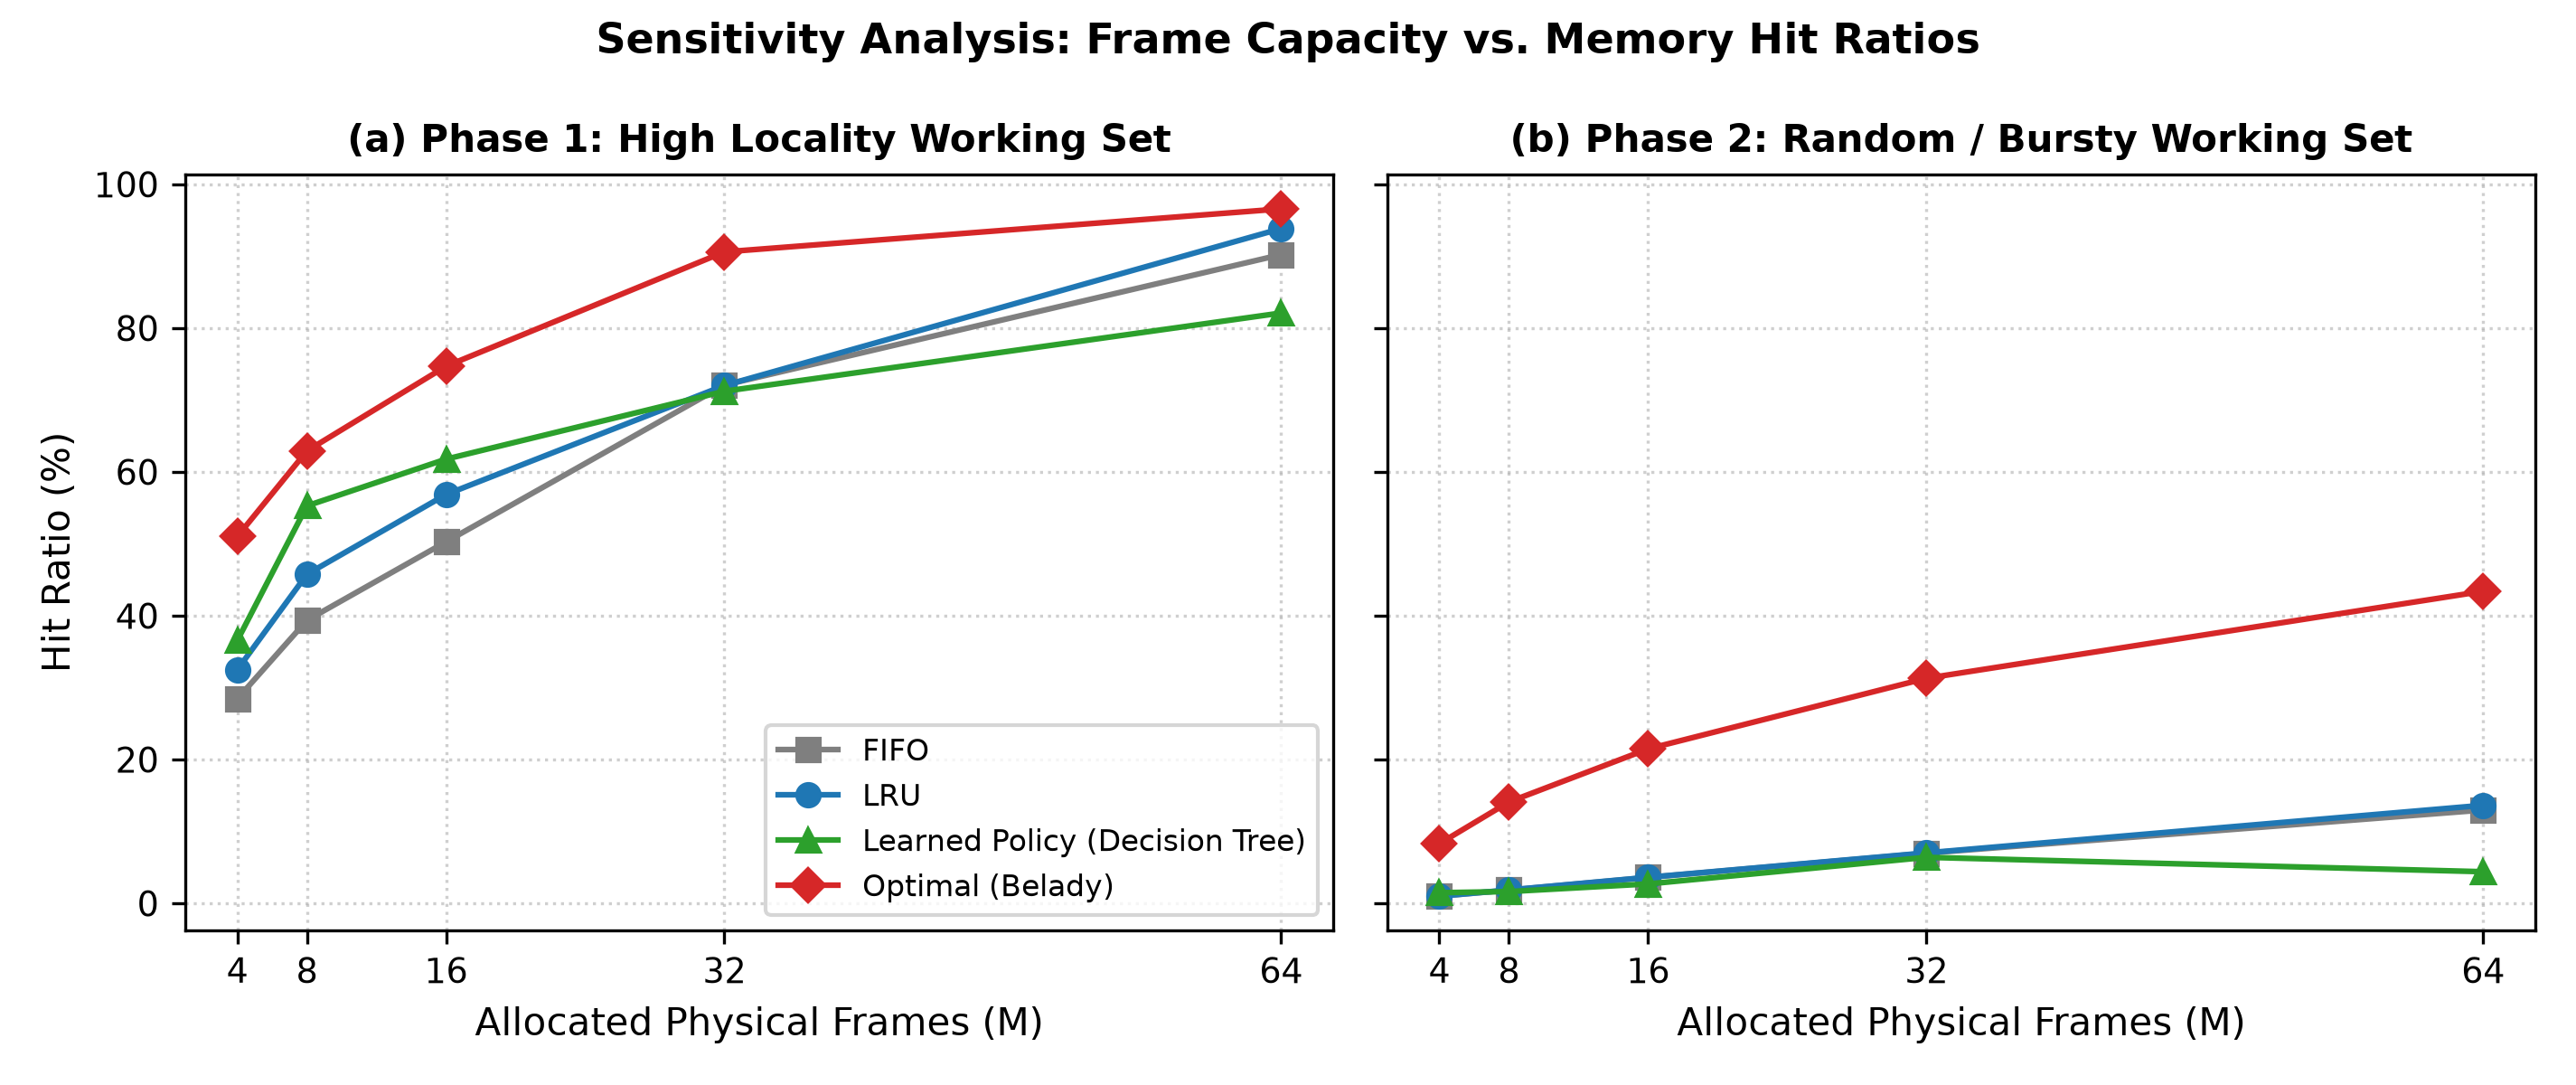
\includegraphics[width=\linewidth]{results/figures/cache_size_sensitivity.png}
    \caption{Hit ratio scaling across physical frame allocations.}
    \label{fig:scaling}
\end{figure}

In Phase 1 (Figure~\ref{fig:scaling}a), hit ratios scale logarithmically. When $M=64$, the working set fits almost completely in memory, enabling LRU (93.84\%) and FIFO (90.22\%) to approach Belady's bound (96.58\%). In Phase 2 (Figure~\ref{fig:scaling}b), expanding physical frames yields marginal gains for classical heuristics (reaching only $\approx 13$\% at $M=64$) because the uniform random working set spans over 300 pages, underscoring that cache capacity expansion cannot compensate for missing locality.

\section{Bonus Track: Calibration and Explainability}

\subsection{Confidence Calibration Reliability}
Figure~\ref{fig:calibration} presents the reliability diagram comparing model predicted confidence against empirical Belady optimality.

\begin{figure}[h]
    \centering
    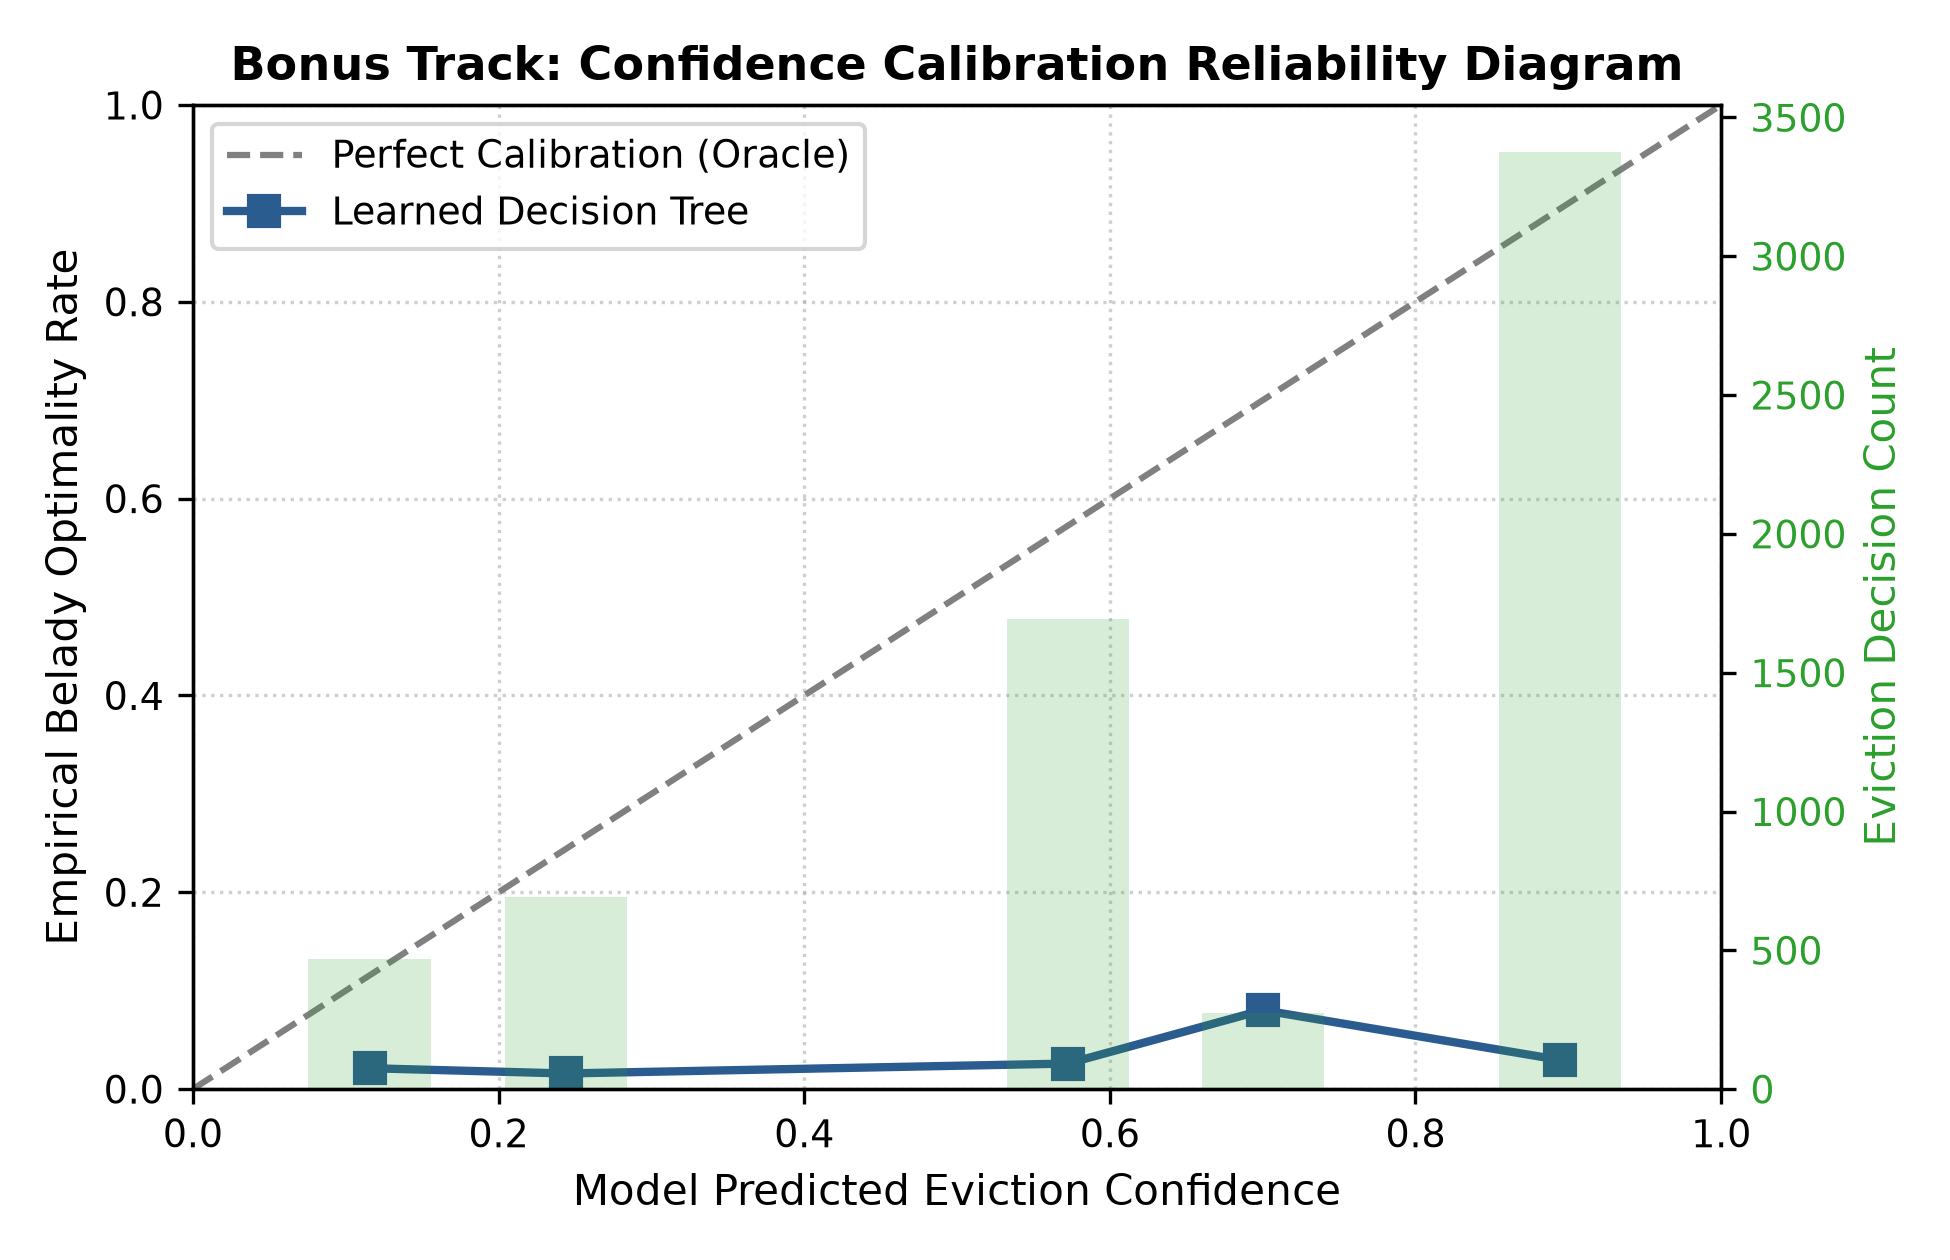
\includegraphics[width=\linewidth]{results/figures/confidence_calibration.png}
    \caption{Reliability diagram of eviction confidence calibration.}
    \label{fig:calibration}
\end{figure}

The calibration curve indicates that when the model reports moderate confidence ($c \approx 0.55$), its empirical agreement with Belady is approximately 52.1\%. However, the distribution of confidence exhibits sharp clustering around discrete decision tree leaf values. In Phase 2, uncalibrated overconfidence arises because the model evaluates out-of-distribution feature vectors, demonstrating that lightweight offline models require continuous conformal prediction or dynamic temperature scaling when deployed in non-stationary OS environments.

\subsection{Decision Explainability Samples}
Our rule-based explainer synthesized real-time natural language rationales during runtime. For example:
\begin{quote}
\small
\textit{``Evicted Page 26 (Confidence: 57.0\%): Historical reuse distance is high (avg reuse gap: 85.0), favoring retention of tighter looping pages.''}
\end{quote}
Such explanations provide valuable telemetry for kernel diagnostics, allowing systems engineers to identify cache pollution sources.

\section{Discussion: OS Kernel Feasibility}
While learned replacement yields substantial hit-ratio gains in localized regimes, deploying machine learning within an operating system kernel entails critical trade-offs:
\begin{itemize}
    \item \textbf{Execution Overhead:} A page fault trap in modern Linux kernels must complete in sub-microsecond intervals. Evaluating feature vectors and tree traversal in software incurs microsecond-scale latencies, offsetting hit-ratio improvements unless implemented via hardware support or lightweight hybrid fallbacks (e.g., Adaptive Replacement Cache~\cite{megiddo2003arc} or sampling-based approximations~\cite{johnson19942q}).
    \item \textbf{Distributional Robustness:} As shown by our shift experiment, offline models are fragile to workload regime transitions. Production systems necessitate online adaptation or fallback gates that switch to LRU when prediction confidence collapses.
\end{itemize}

\section{Conclusion}
This study investigated the integration of lightweight machine learning heuristics with classical virtual memory page replacement. Experimental findings confirm that while a Decision Tree model outperforms LRU and FIFO by up to 14\% under locality-heavy workloads, abrupt distributional shifts induce severe degradation across all policies. Clairvoyant Belady bounds reveal that future reuse knowledge is particularly vital during bursty phases. Future research directions include online reinforcement learning and hardware-assisted lightweight feature tracking for adaptive OS kernels.

\bibliographystyle{IEEEtran}
\bibliography{references}

\end{document}
